\section{Ejercicio 2}

\subsection{Introducción}

\noindent Este ejercicio consiste en resolver el problema que busca el MCS entre dos grafos con un algoritmo exacto. Este es un problema de tipo NP-completo. Más adelante calcularemos la complejidad exacta y luego desarrollaremos diferentes heurísticas basadas en metaheurísticas polinomiales, que a pesar de que no aseguran un resultado exacto, a veces pueden resultar convenientes ya que la diferencia de tiempos es muy notable.

\subsection{Implementación}

\noindent El algoritmo recibe dos grafos y se quiere hallar al máximo subgrafo común entre ellos. Sea $G1$ el grafo que tiene la menor cantidad de nodos y $G2$ el otro grafo. Si ambos tienen igual cantidad de nodos es indistinto cuál es $G1$ y cuál es $G2$.\\

\noindent El algoritmo funciona de la siguiente forma: 
\begin{itemize}
\item Primero notemos que el grafo solución va a tener la misma cantidad de nodos que el grafo $G1$. Esto se encuentra justificado en el $Lema 1$.
\item Ahora se quiere maximizar la cantidad de aristas que podemos encontrar entre los dos grafos, tomando como cantidad de nodos, la cantidad de nodos de $G1$. \\
Para ello utilizamos un vector $mapeo$ en el cual cada posición representa un nodo del grafo $G1$ (la posición $i$ representa el nodo del subgrafo común al cual mapeamos el nodo $i$ del grafo $G1$, con 0 $\leq$ $i$ $<$ $cantidad$ $de$ $nodos$ $de$ $G1$) y el valor de esa posición será el nodo que se corresponde con éste en $G2$ (el nodo $i$ de $G1$ se corresponde con el nodo $vector[i]$ de $G2$).
\begin{figure}[H]
\centering
\begin{subfigure}[h]{0.2\textwidth}
  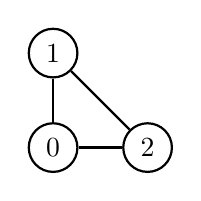
\begin{tikzpicture}[scale= 0.6]
  \node[draw,circle,thick](0) at (0,0){0}; \\
   \node[draw,circle,thick](1) at (0,2){1}; \\
   \node[draw,circle,thick](2) at (2,0){2}; \\
  % \draw [thick,->] (a) to [out=120,in=180] (b);
   \draw [thick] (0) -- (1);
   \draw [thick] (1) -- (2);
   \draw [thick] (0) -- (2);
  \end{tikzpicture}
\caption{$G1$}
 \end{subfigure}
\begin{subfigure}[h]{0.2\textwidth}
  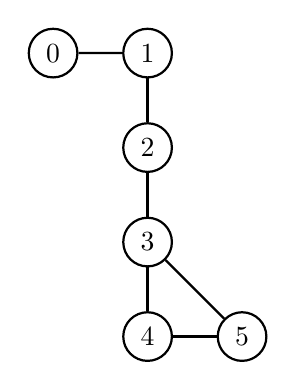
\begin{tikzpicture}[scale= 0.6]
  \node[draw,circle,thick](0) at (-2,6){0}; \\
   \node[draw,circle,thick](1) at (0,6){1}; \\
   \node[draw,circle,thick](2) at (0,4){2}; \\
    \node[draw,circle,thick](3) at (0,2){3}; \\
   \node[draw,circle,thick](4) at (0,0){4}; \\
   \node[draw,circle,thick](5) at (2,0){5}; \\

  % \draw [thick,->] (a) to [out=120,in=180] (b);
   \draw [thick] (0) -- (1);
   \draw [thick] (1) -- (2);
   \draw [thick] (2) -- (3); 
   \draw [thick] (3) -- (4);
   \draw [thick] (3) -- (5);
   \draw [thick] (4) -- (5);
  \end{tikzpicture}
\caption{$G2$}
\end{subfigure}
\end{figure}

\begin{figure}[H]
\centering
\begin{subfigure}[H]{0.4\textwidth}

\begin{table}[H]
\centering Mapeo
\label{my-label}
\begin{tabular}{ccc}
\hline
\multicolumn{1}{|c|}{\textbf{3}} & \multicolumn{1}{c|}{\textbf{4}} & \multicolumn{1}{c|}{\textbf{5}} \\ \hline
0                                & 1                               & 2                              
\end{tabular}
\end{table}
\end{subfigure}
\begin{subfigure}[H]{0.4\textwidth}


\begin{table}[H]
\centering
\label{my-label}
\begin{tabular}{clc}
\textbf{Aristas de $G1$} & \multicolumn{1}{c}{\textbf{}}         & \textbf{Aristas de $G2$} \\
(0,1)                  & $\leftrightarrow$ & (3,4)                  \\
(1,2)                  & $\leftrightarrow$                    & (4,5)                  \\
(2,0)                  & $\leftrightarrow$                     & (5,3)                 
\end{tabular}
\end{table}

\end{subfigure}
\caption{Ejemplo de mapeo}
\end{figure}


\item Luego comparamos la cantidad de aristas que se obtienen en cada mapeo posible, y nos quedamos con el que más tenga. 
\end{itemize}

\subsubsection*{Lema 1}
\noindent Sea $G1$ y $G2$ dos grafos donde $G1$ es el que tiene menor cantidad de nodos. Sea $G'$ un subgrafo común con la mayor cantidad de aristas posibles, y si hay más de uno entonces tomamos uno que tenga la mayor cantidad de vértices posibles, entonces $G'$ tiene la misma cantidad de nodos que $G1$. \\
$\mathbf{Demostraci\acute{o}n:}$ \\
\noindent Sea $G'$ el grafo definido en el enunciado del lema. Supongamos que $G'$ tiene menor cantidad de nodos que $G1$. Entonces si agrego un nodo más a $G'$ sin conectarle aristas sigue siendo subgrafo de $G1$ y por lo tanto de $G2$ también ya que $G2$ tiene mayor o igual cantidad de nodos que $G1$. Entonces $G'$ no era máximo en nodos. Absurdo. El absurdo viene de suponer que $G'$ puede tener menos nodos que $G1$. \\
Supongamos ahora que $G'$ tiene mayor cantidad de nodos que $G1$. Entonces $G'$ no es subgrafo de $G1$ ya que una de las condiciones para ser subgrafo es que el conjunto de nodos de $G'$ tiene que estar incluido en el de $G1$. Absurdo. El absurdo viene de suponer que $G'$ puede tener más nodos que $G1$.\\
Entonces como $G'$ no puede tener ni mayor ni menor cantidad de nodos que $G1$, entonces $G'$ tiene igual cantidad de nodos que $G1$. A los fines de este trabajo práctico escribiremos soluciones que encuentren subgrafos comunes que sean máximos en aristas y que tengan la misma cantidad de nodos que $G1$.\\


\begin{algoritmo}{MCS}{vector(int) mapeo, vector(vector(int)) grafoChico, vector(vector(int)) GrafoGrande }{void}

	\If(\com*{en maximaCantidadDeAristasPosibles se tiene la cantidad de aristas del grafoChico, el MCS no puede superar esta cantidad. Esta es la poda, ya que corta el algoritmo si llega a un resultado insuperable por mas de que no se hayan recorrido todos los mapeos posibles.}){CantidadAristasMejorSolucionHastaElMomento == maximaCantidadDeAristasPosibles}{
return \;
	}
	\For{(cadaMapeoPosible)}{

    	\If{la nueva solución es mejor que la que tengo guardada en CantidadAristasMejorSolucionHastaElMomento}{ 
    		aristasMejorSolucion = aristasDeLaNuevaSolución
    		CantidadAristasMejorSolucionHastaElMomento = CantidadDeAristasDeLaNuevaSolución
   		}
    MCS(mapeo,grafoChico,grafoGrande);
    }
\end{algoritmo}



\subsection{Complejidad}
Para calcular la complejidad de este algoritmo primero analizaremos la complejidad del mismo sin tener en cuenta la poda y luego verificaremos que la poda no empeora la complejidad del mismo.\\
La notación a utilizar será correspondiente a la utilizada anteriormente: los grafos serán $G1$ y $G2$ donde 
$\# V(G1) = n_1$, 
$\# A(G1) = m_1$ y 
$\# V(G2) = n_2$, 
$ \# A(G2) = m_1$ 
con $n_1 \leq n_2$.\\
Analizaremos entonces la complejidad del algoritmo despreciando la poda. Observamos para esto que el algoritmo se resume a: 
\begin{itemize}
	\item Recibir los parámetros de entrada.
	\item Aplicar la función MCS.
    \item Mostrar el resultado%, es decir, que la complejidad del algoritmo se vera en esta función.
\end{itemize}

Con esta observación podemos asegurar que la complejidad total del algoritmo estará dada por la cantidad de veces que se ejecuta la función $MCS(..)$, multiplicado por la complejidad de cada ejecución , es decir, la complejidad de la función en cada llamado multiplicado por la cantidad de llamadas.\\
Distinguimos que la complejidad de la ejecución de la función $MCS(..)$ depende si se la esta llamando con un mapeo (el vector mapeo) completo o uno incompleto, es decir, si el vector tiene el tamaño $n_1$ o si es mas chico. Analizaremos ambos casos por separado:

\begin{enumerate}[(a)]
  
\item Si se la está llamando con un mapeo completo, el algoritmo tarda $\mathcal{O}((n_1 + m_1)*m_2)$ como cota pues es lo que se tarda en recorrer G1 (y a la vez el vector ``mapeo'') y para cada nodo allí preguntar en $\mathcal{O}(m_2)$ qué aristas tienen en común con un vértice particular de G2 (dicho vértice lo determina ``mapeo''; observemos que si bien $G2$ tarda $\mathcal{O}(n_2+m_2)$ en recorrerse, al ya tener el índice del nodo a consultar sólo se recorren sus vecinos, que son a lo sumo $m_2$ y no es necesario el $n_2$ dado que no se recorren todos los nodos, sino sólo el indicado por ``mapeo''). En esta complejidad quedan absorbidos también los costos de comparar con el mejor mapeo hasta el momento y los costos de copiarlo en caso de ser el ``nuevo mejor mapeo'', ya que éstos son subgrafos de $G1$ y $G2$ así que en particular recorrerlos costará $\mathcal{O}(n_1+m_1)$ por ser $G1$ el más chico de ambos grafos y esto queda absorbido en la complejidad dicha ($\mathcal{O}((n_1 + m_1)*m_2)$).\\
Si uno se permitiese ser menos preciso podría decir que es $\mathcal{O}((n_1+m_1)*n_2^2)$ ya que la cantidad de aristas posibles de $G2$ están limitadas por la cantidad de aristas de $ \# A(K_{n_2}) \in \mathcal{O}(n_2^2)$ (esto último es por propiedad enunciada en las teóricas y prácticas), y perdiendo aún más precisión, usando la misma propiedad podría simplificarse a $\mathcal{O}((n_1+n_1^2)*n_2^2) = \mathcal{O}(n_1^2*n_2^2)$ y por último, como $n_1 \leq n_2$ a $\mathcal{O}(n_2^4)$. Estas simplificaciones son útiles para tener un visión panorámica a gran escala de la complejidad, pero por precisión, en el desarrollo que sigue usaremos la complejidad más precisa de $\mathcal{O}((n_1 + m_1)*m_2)$.
\item Si en cambio se la está llamando con un vector de mapeo incompleto, es decir, de tamaño menor estricto a $n_1$, entonces se procede a mapear uno mas, lo que tiene complejidad $\mathcal{O}(n_1)$ ya que para mapear uno mas (digamos que se quiere mapear el nuevo vértice $v_1$ de $G1$ al vértice $v_j$ de $G2$), se debe recorrer el vector ``mapeo'' y chequear que no haya otro ya mapeado al $v_j$, y una vez que verifica esto, realizar un push$\_$back() en 'mapeo', que se puede hacer ya que el vector mapeo tiene tamaño a lo sumo $n_1 - 1$, pues sino hubiese entrado en la opción $(a)$. La complejidad en este caso (en todo $(b)$) es $\mathcal{O}(n_1)$ que es la complejidad de recorrer el vector para chequear no repetir e insertar uno atrás.\\
\end{enumerate}

\noindent Sabemos, entonces, que cada llamada a $MCS(..)$ tendrá complejidad $\mathcal{O}((n_1 + m_1)*m_2)$ si se la llama con un mapeo completo (por $(a)$) y $\mathcal{O}(n_1)$ si se la llama con un mapeo incompleto (por $(b)$).\\
A continuación analizaremos la cantidad de veces que es llamada la función con parámetros de tipo $(a)$ y cuántas veces es llamada la función con parámetros de tipo $(b)$\\
Contaremos la cantidad de veces que se llama a la función con parámetros del tipo (a) primero:

\begin{itemize}
\item Para estar en el caso (a), el vector ``mapeo'' debe estar completo en sus $n_1$ posiciones con números de $0$ a $n_2 - 1$ (que representan a los vértices correspondientes a $G2$) todos distintos entre sí.
\item Observemos cuántas formas hay de llenar el vector cumpliendo con las condiciones del ítem anterior:\\

\begin{itemize}
\item Para la primer posición (la de índice $0$) hay $n_2$ posibilidades.
\item Para la segunda posición (índice $1$) hay $n_2 - 1$ posibilidades (porque no puedo repetir).
\item Para la posición $i$, en general hay $n_2-i$ posibilidades.
\item Para la última posición (índice $n_1-1$) habrá $n_2-n_1+1$ posibilidades.
\end{itemize}

\item Entonces observamos que la cantidad total de veces que se llamará al caso (a) será:
$n_2 * (n_2-1)*.....(n_2-i)....(n_2-(n_1-1))$ $\leq n_2 * n_2 * n_2*...........*n_2 \leq n_2^{n_1}$
\end{itemize}

Veremos ahora la cantidad de veces que se llama a la función con parámetros de tipo (b). Observemos que éstos son los pasos previos a cada construcción del tipo (a). En un principio hay una primer llamada de tipo (b) la cual realiza $n_2$ (una por cada número que es posible poner del 1 al $n_2$) llamadas, que a su vez realizan $n_2-1$ llamadas cada y así sucesivamente hasta que eventualmente se llegan a los casos tipo (a) y termina.\\
Esta sucesión de llamadas podría entenderse con el siguiente árbol:
    \begin{figure}[H]
      \includegraphics[height=10cm]{graficos/arbolesTipoAyB.jpg}
       \caption{Árbol de llamadas a MCS}
	\end{figure}
Se puede observar que es un árbol ``$n_2-ario$'' (las comillas están pues no es $n_2-ario$ ya que en cada nivel se baja en 1 el grado de cada nodo, pero en términos de complejidad es la misma por la misma justificación que usamos para contar los tipo(a)) completo de altura $n_1$. Como ya habíamos observado, la cantidad de veces que se ejecuta como tipo (a) es $\mathcal{O}(n_2^{n_1})$, que es la cantidad de hojas, mientras que la cantidad de veces que se ejecute como tipo (b) será la cantidad de nodos internos de éste árbol, que es orden de la cantidad de nodos de un $n_2-ario$ completo de $n_1 - 1$ de altura, que puede acotarse por $\mathcal{O}(n_2^{n_1})$.\\

Ya sabemos que se llaman $\mathcal{O}(n_2^{n_1})$ tanto a las ejecuciones tipo (a) como a las tipo (b), y además sabemos que las tipo (a) tiene complejidad $\mathcal{O}((n_1 + m_1)*m_2)$ mientras que las tipo (b) $\mathcal{O}(n_1)$. \\
Concluimos entonces que la complejidad total del algoritmo será $\mathcal{O}(n_2^{n_1}*((n_1 + m_1)*m_2)+n_2^{n_1}*n_1) = \mathcal{O}(n_2^{n_1}*(n_1 + m_1)*m_2) $.
\\ \\
Sólo quedaría ver que la poda no empeora esta complejidad, y no lo hace pues sólo realiza operaciones $\mathcal{O}(1)$ y su código esta comprendido dentro de las ejecuciones tipo (a) y (b), por lo que no aporta a la complejidad total, ya que ese $\mathcal{O}(1)$ es absorbido por las complejidades de las ejecuciones (a) o (b).
 
\subsection{Experimentación}
\noindent El algoritmo toma dos grafos para calcular el máximo subgrafo común, entonces para tomar las mediciones y determinar el tiempo de cómputo de la heurística, generalmente, se modificarán únicamente las cantidades de nodos y aristas de uno de ellos. \\
Sea $n_1$ y $m_1$ la cantidad de nodos y aristas del grafo que se modificará para tomar las mediciones respectivamente, y $n_2$, $m_2$ la cantidad de nodos y aristas del grafo al que se le dejarán constantes las cantidades de nodos y aristas, aunque en cada caso podrán utilizarse grafos distintos por con la misma cantidad de vértices y de aristas.
    
\subsubsection*{Experimento 1}\;
\noindent  El objetivo de este experimento fue extraer conclusiones acerca de la variación en el tiempo de cómputo requerido por el algoritmo para distintos valores de $m_1$, con el fin de determinar su complejidad, dejando $n_1$ fijo. \\
\noindent Para ello se utiliza un generador de grafos que funciona de la siguiente manera: dada una cantidad de nodos y aristas, en cada paso crea una nueva arista con extremos válidos (es decir, entre 0 y la cantidad de nodos - 1) y que no este repetida (que no haya sido creada todavía).
     	
\subsubsection*{Datos de entrada}\;
   		\noindent Para correr el algoritmo con poda los valores de $m_1$ tomados fueron desde $0$ hasta $28$ de $2$ en $2$. Como es un algoritmo que resuelve un problema de tipo NP-completo no se pudieron utilizar valores grandes ya que el tiempo de ejecución es muy alto. El valor de $n_1$ fue $8$.\\
       Los valores de $n_2$ y $m_2$ fueron $8$ y $17$ respectivamente. Estos valores fueron elegidos de forma arbitraria teniendo en cuenta que no se pueden utilizar números muy altos por las razones explicadas anteriormente\\
        Para generar los grafos de forma aleatoria se utilizó el generador-grafo-rapido.cpp que se encuentra en la carpeta src y para correrlo se utilizó el exp1.sh que se encuentra en la carpeta exp/ejercicio2/exp1. \\
        Para el caso del que no tiene poda se corrió el algoritmo con los mismos valores de $n_1$, $m_1$, $n_2$ y $m_2$ que en el caso anterior y se utilizó el mismo generador de grafos aleatorios. Para correrlo se utilizó el exp1.sh que se encuentra en la carpeta exp/ejercicio2/exp1bis.\\
        Con el fin de acercarse a los valores reales y descartar posibles falsos resultados, se ejecuta la resolución del problema para cada una de los valores de $m_1$ siete veces considerando luego el promedio entre los valores obtenidos pero graficando también el desvío estándar (la cantidad de repeticiones a realizar fue elegida arbitrariamente).\; 

\subsubsection*{Resultados}\;

    \begin{figure}[H]
      \includegraphics[height=10cm]{graficos/ejercicio2-exp1.png}
       \caption{Experimento 1}
	\end{figure}
    
    \begin{figure}[H]
      \includegraphics[height=10cm]{graficos/ejercicio2-exp1bis.png}
       \caption{Experimento 1 - Sin Poda}
	\end{figure}
\subsubsection*{Observaciones y Conclusiones}\;
En las dos figuras anteriores se puede observar como aumenta el tiempo en relación a lo esperado comportándose como el cálculo de complejidad lo sugiere. En la primer figura se puede observar como la poda efectivamente en algunos casos reduce el tiempo de ejecución (aunque no así la complejidad asintótica) en comparación con el algoritmo sin poda (segunda figura).\\
Concluimos que el experimento demuestra el comportamiento esperado en cuanto a variar la cantidad de aristas de G1 ($m_1$).\\

        
\subsubsection*{Experimento 2}\;
\noindent Este experimento es similar al anterior, pero ahora se va a variar la cantidad de nodos. Para ello, para cada cantidad de nodos se definirá una función para determinar la cantidad de aristas que tendrá el grafo. \\
\noindent Se tuvieron en cuenta 4 funciones, con el fin de que el grafo obtenido no sea siempre uno especial y de esta forma poder analizar diferentes casos.
        \begin{itemize}
        \item F1($n_1$) = $n_1$($n_1$-1))/2 = $m_1$ 
        \item F2($n_1$) = $n_1$-1 = $m_1$ 
        \item F3($n_1$) = 3$n_1$ = $m_1$ 
        \item F4($n_1$) = $n_1^{2}$/10 = $m_1$ 
		\end{itemize} 
Para generar los grafos con estas cantidades de aristas y nodos se utilizó el mismo generador que en el experimento anterior.

\subsubsection*{Datos de entrada}\;
\noindent Los valores de $n_1$ tomados fueron desde $1$ hasta $7$. Como es un algoritmo que resuelve un problema de tipo NP-completo no se pudieron utilizar valores grandes ya que el tiempo de ejecución es muy alto.\\
       Los valores de $n_2$ y $m_2$ fueron $10$ y $20$ respectivamente. Estos valores fueron elegidos de forma arbitraria teniendo en cuenta que no se pueden utilizar números muy altos por las razones explicadas anteriormente\\
        Para generar los grafos de forma aleatoria se utilizó el generador-grafo-rapido.cpp que se encuentra en la carpeta src y para correrlo se utilizó el exp2.sh que se encuentra en la carpeta exp/ejercicio2/exp2. \\
        Con el fin de acercarse a los valores reales y descartar posibles falsos resultados, se ejecuta la resolución del problema para cada una de los valores de $n_1$ cinco veces considerando luego el promedio entre los valores obtenidos pero graficando también el desvío estándar (la cantidad de repeticiones a realizar fue elegida arbitrariamente).\; 

\subsubsection*{Resultados}\;

    \begin{figure}[H]
      \includegraphics[height=10cm]{graficos/ejercicio2-exp2.png}
       \caption{Experimento 2}
	\end{figure}


\subsubsection*{Observaciones y Conclusiones}\;
 \noindent En la figura anterior puede observarse como en todos los casos el algoritmo parece respetar la complejidad propuesta cuando se varía la cantidad de nodos de G1 independientemente de su cantidad de aristas asociadas. Se puede observar también como en algunas circunstancias la poda reduce el tiempo de cómputo.\\
Ciertas simetrías en cuándo la poda es efectiva se pueden observar entre las diferentes F. Atribuimos esta coincidencia al echo de que los grafos a pesar de ser generados con distintas cantidades de aristas, son generados de forma similar.\\
Concluimos de este experimento que el tiempo de ejecución del algoritmo respeta la complejidad propuesta cuando se hace variar la cantidad de nodos del grafo G1.
    
\subsubsection*{Experimento 3}\; 
 \noindent El objetivo de este experimento fue extraer conclusiones acerca de la variación en el tiempo de cómputo requerido por el algoritmo para distintos valores de $m$ y $n$ variando los dos grafos al mismo tiempo pero siempre manteniendo $n_1$ igual a $n_2$ y $m_1$ igual a $m_2$. \\
Para generar los grafos con estas cantidades de aristas y nodos se utilizó el mismo generador que en el experimento anterior. 
        
\subsubsection*{Datos de entrada}\;
\noindent Los valores de $n$ tomados fueron desde $1$ hasta $8$. Como es un algoritmo que resuelve un problema de tipo NP-completo no se pudieron utilizar valores grandes ya que el tiempo de ejecución es muy alto. Para cada $n$ se utilizó $3 \times n$ como cantidad de aristas.\\
        Para generar los grafos de forma aleatoria se utilizó el generador-grafo-rapido.cpp que se encuentra en la carpeta src y para correrlo se utilizó el exp3.sh que se encuentra en la carpeta exp/ejercicio2/exp3. \\
        Con el fin de acercarse a los valores reales y descartar posibles falsos resultados, se ejecuta la resolución del problema para cada una de los valores de $n$ cinco veces considerando luego el promedio entre los valores obtenidos pero graficando también el desvío estándar (la cantidad de repeticiones a realizar fue elegida arbitrariamente).\; 
        
\subsubsection*{Resultados}\;

    \begin{figure}[H]
      \includegraphics[height=10cm]{graficos/ejercicio2-exp3.png}
       \caption{Experimento 2}
	\end{figure}

\subsubsection*{Observaciones y Conclusiones}\;
En la figura anterior puede observarse como el algoritmo parece respetar la complejidad asintótica propuesta, a pesar de estar para n pequeño por arriba de la curva de complejidad, rápidamente se adecua y se sitúa ligeramente por debajo con similar curvatura).\\
Concluimos entonces que el algoritmo respeta la complejidad asintótica propuesta para el caso de variar manteniendo $n_1=n_2$ y $m_1=m_2$.

\subsubsection*{Experimento 4}\;
\noindent  El objetivo de este experimento fue comparar el tiempo de cómputo requerido por el algoritmo con y sin poda. \\
Para ello, para cada cantidad de nodos se definirá una función para determinar la cantidad de aristas que tendrá el grafo. \\
Se tuvieron en cuenta 2 funciones, con el fin de que el grafo obtenido no sea siempre uno especial y de esta forma poder analizar diferentes casos. Las funciones utilizadas son F3 y F4, ya definidas en el experimento 2, ya que son las dos que no generan grafos especiales, como sí es el caso de F1 y F2.
Para generar los grafos con estas cantidades de aristas y nodos se utilizó el mismo generador que en el experimento 1. 
     	
\subsubsection*{Datos de entrada}\;
\noindent Los valores de $n_1$ tomados fueron desde $1$ hasta $7$. Como es un algoritmo que resuelve un problema de tipo NP-completo no se pudieron utilizar valores grandes ya que el tiempo de ejecución es muy alto. Los valores de $m_1$ están definidos por las funciones F3 y F4.\\
       Los valores de $n_2$ y $m_2$ fueron $10$ y $20$ respectivamente. Estos valores fueron elegidos de forma arbitraria teniendo en cuenta que no se pueden utilizar números muy altos por las razones explicadas anteriormente.\\
        Para generar los grafos de forma aleatoria se utilizó el generador-grafo-rapido.cpp que se encuentra en la carpeta src y para correrlo se utilizó el exp4.sh que se encuentra en la carpeta exp/ejercicio2/exp4. \\
        Con el fin de acercarse a los valores reales y descartar posibles falsos resultados, se ejecuta la resolución del problema para cada una de los valores de $n_1$ cinco veces considerando luego el promedio entre los valores obtenidos pero graficando también el desvío estándar (la cantidad de repeticiones a realizar fue elegida arbitrariamente).\; 
        
\subsubsection*{Resultados}\;

    \begin{figure}[H]
      \includegraphics[height=10cm]{graficos/ejercicio2-exp4.png}
       \caption{Experimento 2}
	\end{figure}
\subsubsection*{Conclusiones}\;
En la anterior figura puede observarse como la complejidad pareciera darse igual tanto para el algoritmo con poda como para el sin poda. La efectividad de la poda, en algunos casos, reduce notablemente el tiempo de cómputo.\\
Concluimos entonces de este experimento, que las tanto el algoritmo con poda como sin ella tienen la misma complejidad asintótica, aunque la poda es efectiva en algunos casos para reducir el tiempo de computo.
    